\documentclass[11pt,a4paper]{article}
\usepackage{amsmath, amssymb, graphicx, xcolor}

\setlength{\textwidth}{6.8in}
\setlength{\textheight}{9.6in}
\setlength{\oddsidemargin}{-0.15in}
\setlength{\evensidemargin}{-0.15in}
\setlength{\topmargin}{-0.6in}
\setlength{\headheight}{0in}
\setlength{\headsep}{0in}
\setlength{\parindent}{0pt}
\setlength{\parskip}{5pt}

\definecolor{primary}{RGB}{15, 45, 95}
\definecolor{secondary}{RGB}{30, 80, 150}
\definecolor{accent}{RGB}{180, 40, 40}
\definecolor{qboxbg}{RGB}{245, 248, 252}

\newcommand{\questionheader}[3]{
    \vspace{0.35cm}
    \noindent\colorbox{qboxbg}{
        \parbox{\dimexpr\textwidth-2\fboxsep\relax}{
            \textbf{\textcolor{primary}{\large #1}} \hfill \textbf{\textcolor{accent}{[#2]}} \hfill \textbf{\textcolor{secondary}{#3 Marks}}
        }
    }
    \vspace{0.15cm}
}

\newcommand{\sectionbanner}[1]{
    \vspace{0.5cm}
    \noindent\colorbox{primary}{
        \parbox{\dimexpr\textwidth-2\fboxsep\relax}{
            \centering \textbf{\textcolor{white}{\Large #1}}
        }
    }
    \vspace{0.25cm}
}

\begin{document}

\begin{center}
    {\LARGE \textbf{\textcolor{primary}{BRAC UNIVERSITY}}}\\[4pt]
    {\large \textbf{Department of Computer Science and Engineering}}\\[3pt]
    {\textbf{CSE421 / EEE465: Computer Networks --- Final Examination}}\\[2pt]
    \textbf{Semester:} Spring 2026 \quad | \quad \textbf{Set:} B \quad | \quad \textbf{Full Marks:} 70 \quad | \quad \textbf{Duration:} 2 Hours\\[2pt]
    \rule{\textwidth}{1.5pt}
    {\large \textbf{\textcolor{secondary}{COMPREHENSIVE SOLUTION AND COMPLETE ANSWER KEY}}}
    \rule{\textwidth}{0.8pt}
\end{center}

\sectionbanner{SECTION A: MANDATORY QUESTIONS (40 MARKS)}

% =========================================================================
% QUESTION 1
% =========================================================================
\questionheader{Question 1: Network Address Identification \& VLSM Subnetting}{CO3}{3 + 9 = 12}

\textbf{Problem Context:}
The numbers of hosts specified for each network represent only the end devices. A university is assigned the IP address \texttt{103.84.77.219/20}.

\begin{center}
    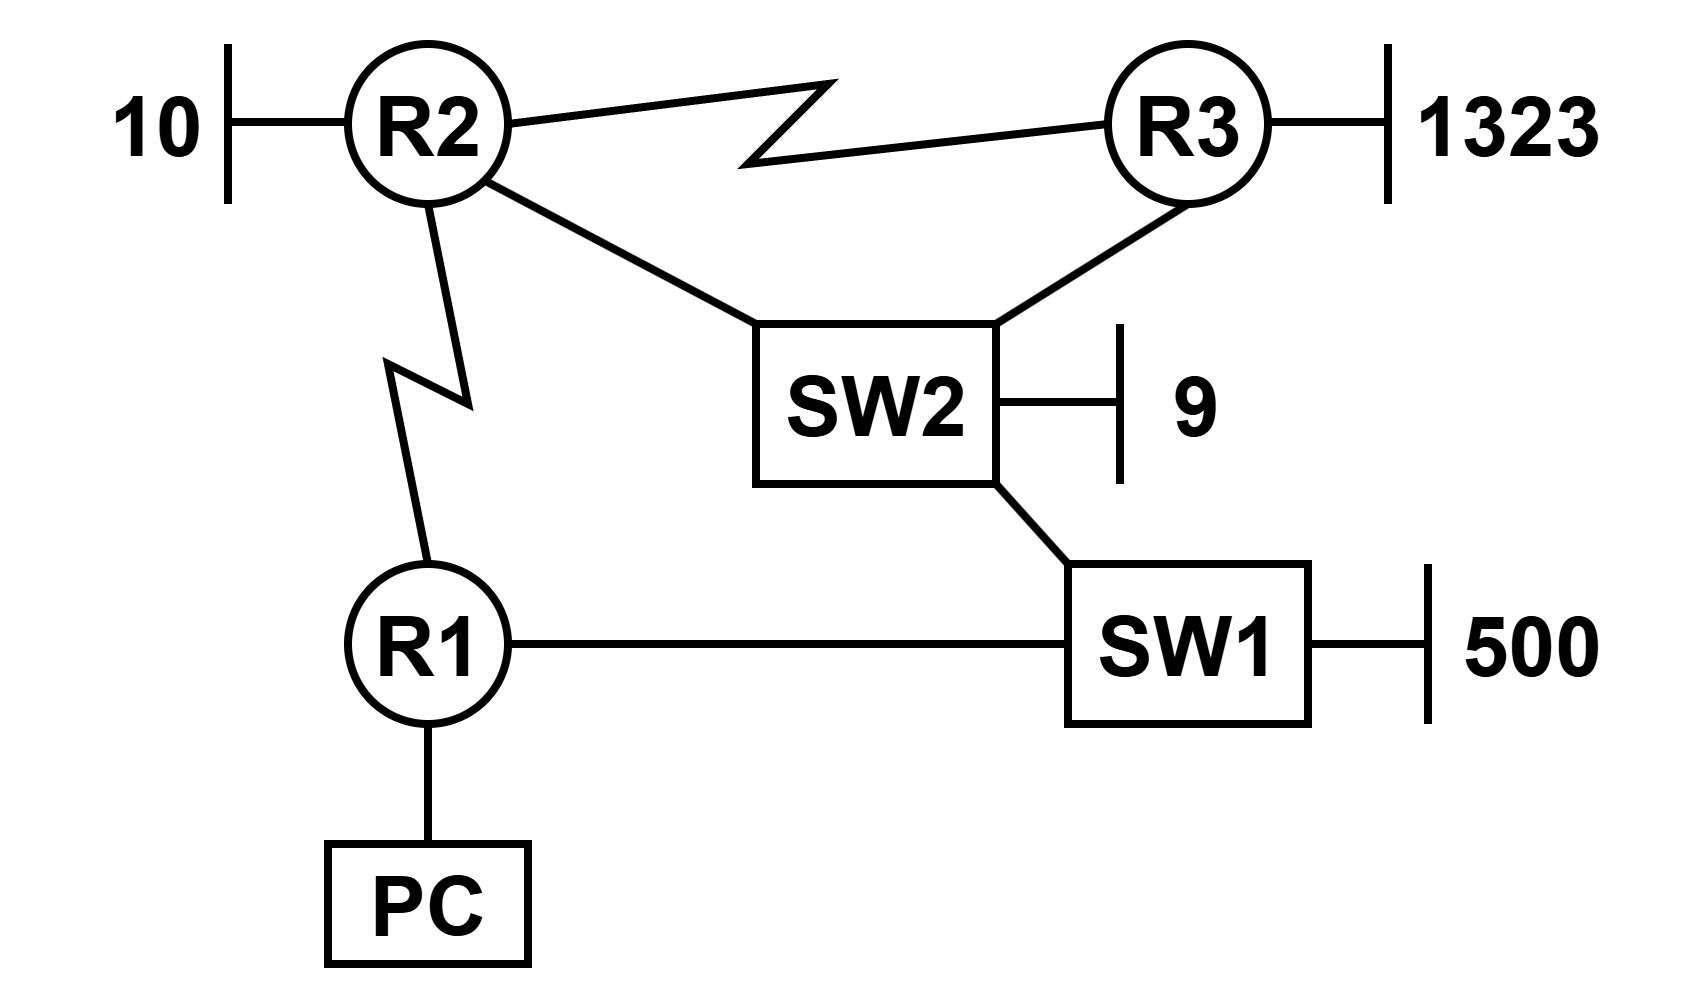
\includegraphics[width=0.45\textwidth]{p5_q1_topology.png}
\end{center}

\textbf{I. Find the network address. [3 Marks]}

\textbf{Solution:}
\begin{itemize}
    \item Given IP address: \texttt{103.84.77.219/20}.
    \item A prefix of $/20$ corresponds to subnet mask:
    \[
    \mathbf{255.255.240.0} \quad (\text{3rd octet binary: } 11110000_2)
    \]
    \item Block size in the 3rd octet is $256 - 240 = 16$.
    \item The 3rd octet value of the given IP is 77.
    \item Finding the multiple of 16 less than or equal to 77:
    \[
    16 \times 4 = 64 \le 77 < 80
    \]
    \item Setting host bits to 0 yields the \textbf{Network Address}:
    \[
    \mathbf{103.84.64.0/20}
    \]
\end{itemize}
\textbf{Answer:} Network Address: \textbf{\texttt{103.84.64.0/20}}.

\vspace{0.2cm}
\textbf{II. VLSM Allocation to Each Network \& Hierarchical Tree. [9 Marks]}

\textbf{Accounting for Router Interfaces:}
\begin{itemize}
    \item R3 LAN: 1323 hosts + 1 gateway = \textbf{1324 IP addresses}.
    \item SW1 LAN: 500 hosts + 1 gateway (R1 interface) = \textbf{501 IP addresses}.
    \item SW2 LAN: 9 hosts + 2 router interfaces (R2, R3) = \textbf{11 IP addresses}.
    \item R2 LAN: 10 hosts + 1 gateway = \textbf{11 IP addresses}.
    \item R1 LAN (PC): 1 host + 1 gateway = \textbf{2 IP addresses}.
    \item WAN Link R1--R2: 2 router interfaces = \textbf{2 IP addresses}.
    \item WAN Link R2--R3: 2 router interfaces = \textbf{2 IP addresses}.
\end{itemize}

\textbf{Allocation in Descending Order:}
\begin{enumerate}
    \item \textbf{R3 LAN (Needs 1324):}
    \begin{itemize}
        \item $2^h - 2 \ge 1324 \implies h = 11$ bits ($2^{11} - 2 = 2046$). Prefix: $/21$ (\texttt{255.255.248.0}). Block size = 8.
        \item \textbf{Subnet Address:} \texttt{103.84.64.0/21}
        \item Usable Range: \texttt{103.84.64.1} -- \texttt{103.84.71.254}; Broadcast: \texttt{103.84.71.255}
        \item Next Available Base: \texttt{103.84.72.0}
    \end{itemize}

    \item \textbf{SW1 LAN (Needs 501):}
    \begin{itemize}
        \item $2^h - 2 \ge 501 \implies h = 9$ bits ($2^9 - 2 = 510$). Prefix: $/23$ (\texttt{255.255.254.0}). Block size = 2.
        \item \textbf{Subnet Address:} \texttt{103.84.72.0/23}
        \item Usable Range: \texttt{103.84.72.1} -- \texttt{103.84.73.254}; Broadcast: \texttt{103.84.73.255}
        \item Next Available Base: \texttt{103.84.74.0}
    \end{itemize}

    \item \textbf{SW2 Multi-Access LAN (Needs 11):}
    \begin{itemize}
        \item $2^h - 2 \ge 11 \implies h = 4$ bits ($2^4 - 2 = 14$). Prefix: $/28$ (\texttt{255.255.255.240}). Block size = 16.
        \item \textbf{Subnet Address:} \texttt{103.84.74.0/28}
        \item Usable Range: \texttt{103.84.74.1} -- \texttt{103.84.74.14}; Broadcast: \texttt{103.84.74.15}
        \item Next Available Base: \texttt{103.84.74.16}
    \end{itemize}

    \item \textbf{R2 LAN (Needs 11):}
    \begin{itemize}
        \item $2^h - 2 \ge 11 \implies h = 4$ bits. Prefix: $/28$ (\texttt{255.255.255.240}). Block size = 16.
        \item \textbf{Subnet Address:} \texttt{103.84.74.16/28}
        \item Usable Range: \texttt{103.84.74.17} -- \texttt{103.84.74.30}; Broadcast: \texttt{103.84.74.31}
        \item Next Available Base: \texttt{103.84.74.32}
    \end{itemize}

    \item \textbf{R1 PC LAN (Needs 2):}
    \begin{itemize}
        \item $2^h - 2 \ge 2 \implies h = 2$ bits. Prefix: $/30$ (\texttt{255.255.255.252}). Block size = 4.
        \item \textbf{Subnet Address:} \texttt{103.84.74.32/30}
        \item Usable Range: \texttt{103.84.74.33} -- \texttt{103.84.74.34}; Broadcast: \texttt{103.84.74.35}
        \item Next Available Base: \texttt{103.84.74.36}
    \end{itemize}

    \item \textbf{WAN Link R1--R2 (Needs 2):}
    \begin{itemize}
        \item Prefix: $/30$ (\texttt{255.255.255.252}).
        \item \textbf{Subnet Address:} \texttt{103.84.74.36/30}
        \item Usable Range: \texttt{103.84.74.37} -- \texttt{103.84.74.38}; Broadcast: \texttt{103.84.74.39}
        \item Next Available Base: \texttt{103.84.74.40}
    \end{itemize}

    \item \textbf{WAN Link R2--R3 (Needs 2):}
    \begin{itemize}
        \item Prefix: $/30$ (\texttt{255.255.255.252}).
        \item \textbf{Subnet Address:} \texttt{103.84.74.40/30}
        \item Usable Range: \texttt{103.84.74.41} -- \texttt{103.84.74.42}; Broadcast: \texttt{103.84.74.43}
    \end{itemize}
\end{enumerate}

\textbf{Hierarchical Subnet Tree:}
\begin{verbatim}
103.84.64.0/20 (Major Network)
 |-- 103.84.64.0/21   [R3 LAN: 1324 Hosts]
 |-- 103.84.72.0/23   [SW1 LAN: 501 Hosts]
 `-- 103.84.74.0/23
      |-- 103.84.74.0/28   [SW2 LAN: 11 Hosts]
      |-- 103.84.74.16/28  [R2 LAN: 11 Hosts]
      |-- 103.84.74.32/30  [R1 PC LAN: 2 Hosts]
      |-- 103.84.74.36/30  [WAN R1-R2: 2 Hosts]
      `-- 103.84.74.40/30  [WAN R2-R3: 2 Hosts]
\end{verbatim}

\newpage
% =========================================================================
% QUESTION 2
% =========================================================================
\questionheader{Question 2: IPv4 Fragmentation Analysis \& Reassembly Requirements}{CO2, CO3}{3 + 2 + 2 + 3 + 3 = 13}

\textbf{Given Parameters:}
\begin{itemize}
    \item Total original datagram size $= 7,340$ bytes (includes 20-byte IP header).
    \item Total payload data $= 7,340 - 20 = 7,320$ bytes.
    \item Link MTU $= 1,300$ bytes.
    \item Max data per intermediate fragment $\le 1,300 - 20 = 1,280$ bytes (divisible by 8: $1280 / 8 = 160$).
    \item Captured fragment: Total Length = 1,300 bytes, $MF = 1$, Fragment Offset = 320.
\end{itemize}

\textbf{I. Which fragment was captured? [3 Marks]}
\begin{itemize}
    \item From the course networking study notes, the Fragment Offset for the $k$-th fragment is given by:
    \[
    \text{Fragment Offset}_k = \frac{(k - 1) \times \text{Payload}}{8}
    \]
    where $k$ is the fragment index ($k = 1, 2, 3, \dots$) and $\text{Payload} = 1280\text{ bytes}$ is the data payload per full fragment.
    \item Given that the captured fragment has $\text{Fragment Offset} = 320$:
    \[
    320 = \frac{(k - 1) \times 1280}{8} = (k - 1) \times 160
    \]
    \item Solving directly for $k$:
    \[
    k - 1 = \frac{320}{160} = 2 \implies k = 2 + 1 = \mathbf{3}
    \]
    \item Therefore, the captured fragment is the \textbf{3rd fragment} ($k = 3$).
\end{itemize}

\textbf{II. How many fragments will be created from the original datagram in total? [2 Marks]}
\begin{itemize}
    \item Number of full 1,280-byte fragments $= \lfloor 7,320 / 1,280 \rfloor = 5$ full fragments.
    \item Data carried in first 5 fragments $= 5 \times 1,280 = 6,400$ bytes.
    \item Data remaining for 6th fragment $= 7,320 - 6,400 = 920$ bytes.
    \item \textbf{Total Fragments Created} $= 5 + 1 = \mathbf{6\text{ fragments}}$.
\end{itemize}

\textbf{III. Total Length field value of the last fragment? [2 Marks]}
\begin{itemize}
    \item $\text{Total Length} = \text{Data Payload} + \text{Header Size} = 920 + 20 = \mathbf{940\text{ bytes}}$.
\end{itemize}

\textbf{IV. Fragment Offset value of the last fragment? [3 Marks]}
\begin{itemize}
    \item As established in Part II, there are 6 fragments in total, so the last fragment is the \textbf{6th fragment} ($k = 6$).
    \item Applying the standard fragment offset formula:
    \[
    \text{Fragment Offset}_6 = \frac{(6 - 1) \times \text{Payload}}{8} = \frac{5 \times 1280}{8} = 5 \times 160 = \mathbf{800}
    \]
    \item (Verification: Preceding 5 fragments carry $5 \times 1280 = 6400$ bytes of data, and in 8-byte units $\frac{6400}{8} = 800$).
\end{itemize}

\textbf{V. What information does the destination host need to correctly reassemble fragments? [3 Marks]}
\begin{enumerate}
    \item \textbf{Stream Identifier Tuple:} The 4-tuple \texttt{(Source IP, Destination IP, Protocol, Identification)} to associate fragments to the specific packet stream.
    \item \textbf{Fragment Offset:} To position each payload in the correct sequential byte slot.
    \item \textbf{Total Length \& Header Length:} To compute the payload size of each fragment.
    \item \textbf{More Fragments (MF) Flag:} To detect the terminal fragment ($MF = 0$) and compute total datagram length.
\end{enumerate}

\newpage
% =========================================================================
% QUESTION 3
% =========================================================================
\questionheader{Question 3: DHCPv4, ARP Across Multi-Hops, PAT, \& Switch Aging}{CO2}{3 $\times$ 5 = 15}

\begin{center}
    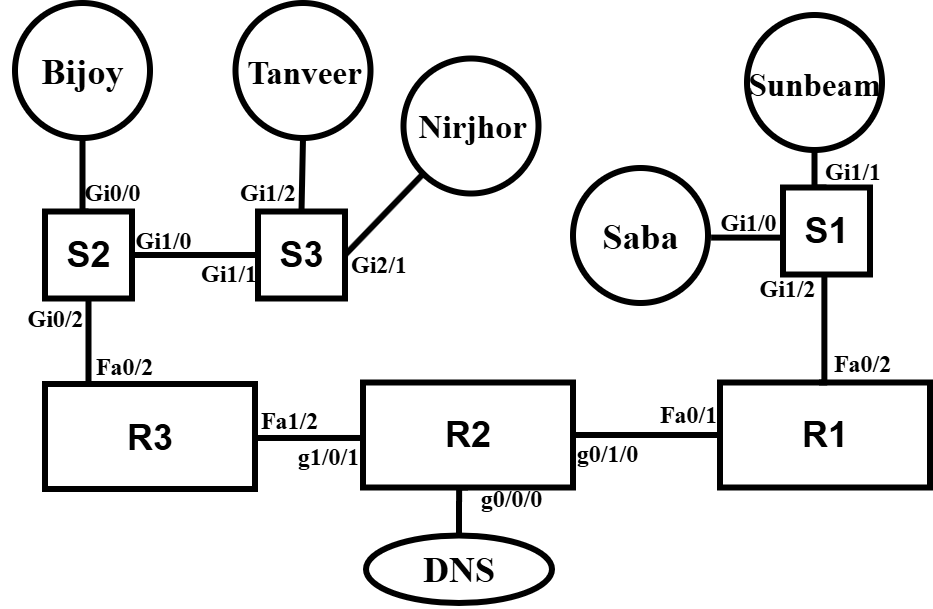
\includegraphics[width=0.75\textwidth]{p5_q3_topology.png}
\end{center}

\textbf{I. Additional information Saba receives from DHCP apart from IP: [3 Marks]}
\begin{enumerate}
    \item \textbf{Subnet Mask} (defining local subnet boundary).
    \item \textbf{Default Gateway IP} (\texttt{10.10.10.1} --- Router R1's interface).
    \item \textbf{DNS Server IP} (\texttt{6.6.6.6}).
    \item \textbf{IP Address Lease Duration} and renewal timers ($T_1, T_2$).
\end{enumerate}

\textbf{II. How R1 distinguishes Sunbeam's and Saba's DHCPDISCOVER requests: [3 Marks]}
\begin{itemize}
    \item \textbf{Client Hardware Address (\texttt{chaddr}):} In the DHCP message payload, Saba sends \texttt{chaddr = SABA} and Sunbeam sends \texttt{chaddr = SUNBEAM}.
    \item \textbf{Transaction ID (\texttt{xid}):} Each client generates a unique 32-bit transaction identifier.
    \item \textbf{Layer 2 Ethernet Header Source MAC:} The Ethernet frame source address contains each host's unique physical MAC address.
\end{itemize}

\textbf{III. Total ARP requests required for Nirjhor to send a packet to Saba: [3 Marks]}
\begin{itemize}
    \item Nirjhor and Saba reside in different broadcast domains across Routers R3, R2, and R1.
    \item Total ARP requests required $= \mathbf{4\text{ ARP Requests}}$:
    \begin{enumerate}
        \item \textbf{ARP Request 1 (Nirjhor's LAN):} Nirjhor broadcasts an ARP request for Default Gateway R3's interface IP.
        \item \textbf{ARP Request 2 (Link R3--R2):} R3 broadcasts an ARP request for R2's receiving interface IP on the shared Ethernet segment.
        \item \textbf{ARP Request 3 (Link R2--R1):} R2 broadcasts an ARP request for R1's receiving interface IP.
        \item \textbf{ARP Request 4 (R1's LAN):} R1 broadcasts an ARP request on its local LAN for Saba's IP address.
    \end{enumerate}
\end{itemize}

\textbf{IV. Can Nirjhor and Saba's DNS requests be uniquely identified by server 6.6.6.6? [3 Marks]}
\begin{itemize}
    \item \textbf{YES, they are uniquely identified.}
    \item \textbf{Explanation:} R3 translates Nirjhor's private IP to R3's public IP \textbf{\texttt{212.9.9.9}}, while R1 translates Saba's private IP to R1's public IP \textbf{\texttt{212.5.5.5}}.
    \item The DNS server receives packets from two completely distinct public IP addresses: \texttt{212.9.9.9:Port1} and \texttt{212.5.5.5:Port2}. The resulting socket pairs are globally unique, enabling the DNS server to process and return replies to each client without ambiguity.
\end{itemize}

\textbf{V. Switch learning after 2 minutes of MAC table expiration: [3 Marks]}
\begin{itemize}
    \item \textbf{Both transmitted frames will cause switches to learn MAC addresses again.}
    \item \textbf{Explanation:} Switch self-learning operates strictly by inspecting the \textbf{Source MAC Address} of incoming frames:
    \begin{enumerate}
        \item Tanveer's ICMP Request has Source MAC \texttt{TANVEER}. Switches S3 and S2 record \texttt{TANVEER} on their respective receiving ports.
        \item Bijoy's ARP Request has Source MAC \texttt{BIJOY}. Switches S2 and S3 record \texttt{BIJOY} on their respective receiving ports.
    \end{enumerate}
\end{itemize}

\newpage
\sectionbanner{SECTION B: ANY TWO OUT OF THREE (12 MARKS)}
\textit{(All questions solved below for complete coverage)}

% =========================================================================
% QUESTION 4
% =========================================================================
\questionheader{Question 4: Traceroute Request Timed Out Analysis}{CO2}{3 + 3 = 6}

\textbf{I. Does intermediate "Request Timed Out" always mean unreachable? [3 Marks]}
\textbf{NO.} If subsequent hops or the final destination respond normally, the destination is completely reachable. Intermediate timeouts simply indicate that specific intermediary routers declined to generate ICMP TTL-exceeded messages.

\textbf{II. Two possible reasons for this behavior: [3 Marks]}
\begin{enumerate}
    \item \textbf{ICMP Rate-Limiting or Firewall Blocking:} Many network administrators configure transit routers or firewalls to drop ICMP Time Exceeded packets to protect router CPU performance and conceal network topology.
    \item \textbf{Asymmetric Routing / Return Path Issue:} The probe packet reached the router, but the return path taken by the router's ICMP response had a temporary routing flaw or upstream filter.
\end{enumerate}

% =========================================================================
% QUESTION 5
% =========================================================================
\questionheader{Question 5: IPv6 Hexadecimal Expansion \& Classification}{CO3}{2 + 4 = 6}

\textbf{I. Expanded Hexadecimal Form [2 Marks]:}
\begin{itemize}
    \item A. \texttt{fdc2:34::ab:0} $\to$ \textbf{\texttt{fdc2:0034:0000:0000:0000:0000:00ab:0000}}
    \item B. \texttt{::1} $\to$ \textbf{\texttt{0000:0000:0000:0000:0000:0000:0000:0001}}
\end{itemize}

\textbf{II. Type \& Internet Routability [4 Marks]:}
\begin{itemize}
    \item \textbf{\texttt{fdc2:34::ab:0}:} Type is **Unique Local Address (ULA)** (prefix \texttt{FC00::/7}, specifically \texttt{FD00::/8}). It is designed for private local communications and is **NOT routable on the public Internet**.
    \item \textbf{\texttt{::1}:} Type is **Loopback Address**. It is restricted to the internal loopback interface of the local host and is **NOT routable on any network or the Internet**.
\end{itemize}

% =========================================================================
% QUESTION 6
% =========================================================================
\questionheader{Question 6: Switch Forwarding \& MAC Table Learning with Bijoy}{CO2}{3 + 3 = 6}

\textbf{Initial Condition:} Only Switch 2 has Bijoy's MAC in its table. Switch 3 does not.

\textbf{I. Tanveer sends a unicast frame to Bijoy: Devices receiving and actions: [3 Marks]}
\begin{enumerate}
    \item \textbf{Switch S3:} Receives frame on \texttt{Gi1/2}, learns Tanveer on \texttt{Gi1/2}. Since Bijoy's MAC is unknown, S3 \textbf{floods} the frame to Nirjhor (\texttt{Gi2/1}) and Switch S2 (\texttt{Gi1/1}).
    \item \textbf{Nirjhor:} Receives frame, inspects Destination MAC (Bijoy), sees mismatch, and \textbf{discards} it.
    \item \textbf{Switch S2:} Receives frame on \texttt{Gi1/0}, learns Tanveer on \texttt{Gi1/0}. S2 has Bijoy's MAC in its table on \texttt{Gi0/0} and \textbf{unicasts} the frame solely to Bijoy.
    \item \textbf{Bijoy:} Receives frame, matches Destination MAC, and \textbf{accepts} it.
\end{enumerate}

\textbf{II. MAC Tables After Bijoy Replies: [3 Marks]}

\begin{center}
\begin{tabular}{|l|c|}
\multicolumn{2}{c}{\textbf{Switch S2 MAC Table}} \\
\hline
\textbf{Device / MAC} & \textbf{Port} \\
\hline
\texttt{BIJOY} & \texttt{Gi0/0} \\
\texttt{TANVEER} & \texttt{Gi1/0} \\
\hline
\end{tabular}
\qquad
\begin{tabular}{|l|c|}
\multicolumn{2}{c}{\textbf{Switch S3 MAC Table}} \\
\hline
\textbf{Device / MAC} & \textbf{Port} \\
\hline
\texttt{TANVEER} & \texttt{Gi1/2} \\
\texttt{BIJOY} & \texttt{Gi1/1} \\
\hline
\end{tabular}
\end{center}

\newpage
\sectionbanner{SECTION C: ANY THREE OUT OF FIVE (18 MARKS)}
\textit{(All questions solved below for complete coverage)}

% =========================================================================
% QUESTION 7
% =========================================================================
\questionheader{Question 7: TTL Bandwidth Impact \& Header Checksum Necessity}{CO2}{3 + 3 = 6}

\textbf{I. Primary Purpose of TTL \& Bandwidth Impact if Omitted: [3 Marks]}
The TTL field prevents packets from being trapped in permanent routing loops. If omitted, looping packets would never expire. As new traffic continuously enters the loop, packets would endlessly accumulate, consuming 100\% of available link bandwidth and causing catastrophic network collapse.

\textbf{II. Why IPv4 has a Header Checksum despite Data-Link Checksums: [3 Marks]}
Routers modify the IPv4 header at each hop (decrementing TTL, changing options, updating checksum). Because the header changes in router memory, Layer 2 CRC (which is stripped upon frame arrival) cannot protect against memory corruption or processing errors inside the router. The IPv4 checksum ensures corrupt headers (especially corrupted destination addresses) are detected and dropped immediately before misrouting.

% =========================================================================
% QUESTION 8
% =========================================================================
\questionheader{Question 8: Link State vs. Distance Vector Mechanics}{CO3}{3 + 3 = 6}

\textbf{I. Continuous Monitoring vs. Periodic Exchange: [3 Marks]}
Link State protocols construct a complete topological map (LSDB) and require instantaneous knowledge of neighbor adjacency state (via Hello packets) to trigger immediate SPF recalculation. Distance Vector routers have no global map and rely purely on the cumulative vector reports sent by neighbors at fixed periodic intervals.

\textbf{II. Why Link State is More Stable \& Adaptive: [3 Marks]}
Link State routers calculate shortest paths independently using Dijkstra's algorithm from an identical, synchronized topological database. This eliminates the ``routing by rumor'' delays, count-to-infinity loops, and slow convergence characteristic of Distance Vector algorithms.

% =========================================================================
% QUESTION 9
% =========================================================================
\questionheader{Question 9: DHCP Relay Scope \& 50\% Lease Renewal Process}{CO2}{3 + 3 = 6}

\begin{center}
    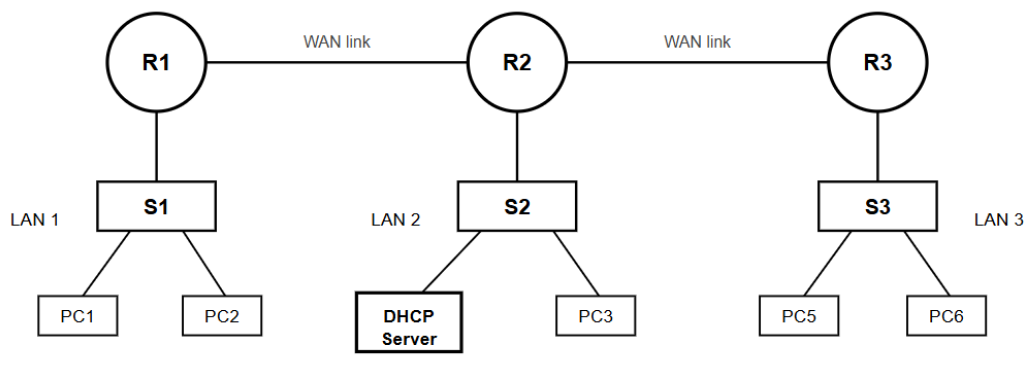
\includegraphics[width=0.7\textwidth]{p5_q9_topology.png}
\end{center}

\textbf{I. Justification of Technician's Claim: [3 Marks]}
\textbf{The claim is INCORRECT.} A DHCP Relay Agent must be configured on the router interface directly serving the client broadcast domain (here, Router R3 for LAN 3). Configuring a relay agent on R1 only forwards DHCP requests originating on R1's LAN; it has no ability to intercept or relay broadcast packets generated behind Router R3.

\textbf{II. DHCP Messages Exchanged at 50\% Lease Elapsed ($T_1$): [3 Marks]}
PC1 enters the \textbf{RENEWING} state and sends a unicast **DHCPREQUEST** message directly to the DHCP server requesting lease extension. The server responds with a unicast **DHCPACK** message confirming the renewed lease time.

% =========================================================================
% QUESTION 10
% =========================================================================
\questionheader{Question 10: Anycast vs. Multicast \& Dual Stack Limitations}{CO2, CO3}{3 + 3 = 6}

\textbf{I. Delivery Logic of Anycast vs. Multicast: [3 Marks]}
\begin{itemize}
    \item \textbf{Anycast (One-to-Nearest):} Routed to \textbf{only one single node} among multiple nodes sharing the address, specifically the topologically closest node according to routing metrics.
    \item \textbf{Multicast (One-to-Many):} Delivered to \textbf{all nodes} that have subscribed to the multicast group.
\end{itemize}

\textbf{II. Why Dual Stack Alone is Insufficient Across IPv4 Transit: [3 Marks]}
Dual Stack requires every router along the transmission path to run IPv6. If the core transit network consists of legacy IPv4-only routers, native IPv6 packets cannot be routed. **IPv6 Tunneling (encapsulation)** is required to encapsulate IPv6 datagrams inside IPv4 packets across the transit network.

% =========================================================================
% QUESTION 11
% =========================================================================
\questionheader{Question 11: Stale ARP Cache \& Switch Transparency}{CO2}{3 + 3 = 6}

\textbf{I. Why the PC cannot print for several minutes after printer NIC replacement: [3 Marks]}
The PC caches the printer's IP-to-MAC mapping in its local **ARP Cache**. When the printer's NIC is replaced, its MAC address changes while its IP remains the same. The PC continues transmitting frames addressed to the old (stale) MAC address until the ARP cache entry times out (typically 2 to 20 minutes depending on OS).

\textbf{II. Why Link-Layer Headers Remain Unchanged Across Interconnected Switches: [3 Marks]}
Switches are Layer 2 transparent bridges that operate by inspecting frame MAC addresses and forwarding them between ports. Unlike Layer 3 routers (which strip and rebuild the link-layer header at every hop), switches never modify the Ethernet frame header or trailer, preserving the sender's original Layer 2 encapsulation end-to-end.

\begin{center}
    \rule{\textwidth}{0.8pt}\\[3pt]
    \textbf{\textcolor{primary}{--- END OF EXAMINATION SOLUTION ---}}
\end{center}

\end{document}
